\section{Basic Agent}
This agent must be able to suck up all dirt in a rectangular world of unknown dimensions without obstacles and shutdown on the stating position (home).

This agent explore the world line by line. When he bump onto a wall, he turn to explore the next line. If, during his turn, he bump again onto a wall, that means that he reach the top (or the bottom) of the world, and that he have to take the way back to home.

After leaving his home, the next time the agent will be on the home cell, he will stop.

We can see an example of exploration in this figure \ref{basicagentexplo1}.

\begin{figure}[ht]
  \centering
  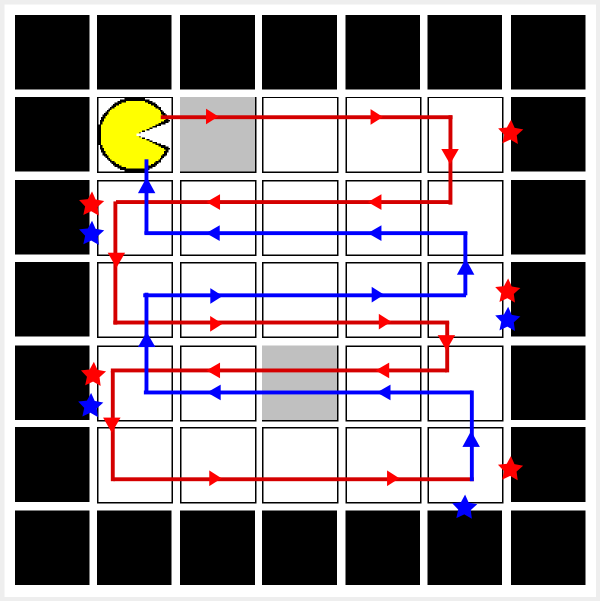
\includegraphics[height=8cm]{img/basicagentexplo1.png}
  \caption{Basic agent exploration (red : exploration, blue : way home, star : bump)}
  \label{basicagentexplo1}
\end{figure} 

As we can see, if the starting position is at any corners of the world, the agent will explore the entire world. But if the starting position is in the anywhere in the middle of the world, this agent will forget to explore all the line which are above the starting position.

\subsection{Results}
In a 5x5 environment with a dirt probability of 10\%, this agent will score 134 (best score for random and reactive vacuum agent is -898)

In a 20x20 environment with a dirt probability of 10\%, this agent will score 3124 (average score for random vacuum agent is -400 and 600 for reactive vacuum agent)

In a 20x20 environment with a dirt probability of 50\%, this agent will score 19124 (average score for random vacuum agent is 600 and 1700 for reactive vacuum agent)

As we can see, this basic agent have better score than the random vacuum agent and the reactive vacuum agent. Which is understandable because this basic agent always go back to home and always stuck all the dirt.

\subsection{Conclusion}
Supposing the starting position is in a corner, this simple agent will explore the entire world, sucking all the dirts.
He will explore the world twice, it's maybe a way where it can be optimized.

This agent could not explore a world with obstacle. Because sometimes this agent will do great work if the obstacle are suitable for its exploration, but mostly, this agent will be trapped in a small part of the world.

